% Emacs, this is -*-latex-*-

\ex{Directed graph concepts}
\label{ex:directed-graph-concepts}
Consider the following directed graph:

\begin{center}
    \scalebox{1}{ % x,y
      \begin{tikzpicture}[dgraph]
        \node[cont] (a) at (0,2) {$a$};
        \node[cont] (z) at (2,2) {$z$};
        \node[cont] (q) at (1,1) {$q$};
        \node[cont] (e) at (1,-0.4) {$e$};
        \node[cont] (h) at (3,1) {$h$};
        \draw(a) -- (q);
        \draw(z) -- (h);
        \draw(z) -- (q);
        \draw(q) -- (e);
    \end{tikzpicture}}
  \end{center}

\begin{exenumerate}
\item List all trails in the graph (of maximal length)

  \begin{solution}
    We have
  $$(a,q,e) \quad \quad (a,q,z,h) \quad \quad  (h,z,q,e)$$
    and the corresponding ones with swapped start and end nodes.
  \end{solution}
    
\item List all directed paths in the graph (of maximal length)
  \begin{solution}
$(a,q,e) \quad \quad (z,q,e) \quad \quad (z,h) $
  \end{solution}
  
\item What are the descendants of $z$?
  
  \begin{solution}
$\desc(z) =\{q,e,h\}$
  \end{solution}

  
\item What are the non-descendants of $q$?
    
  \begin{solution}
$\nondesc(q) = \{a,z,h,e\} \setminus \{e\} = \{a,z,h\}$
  \end{solution}

  
\item Which of the following orderings are topological to the graph?
  \begin{itemize}
    \item (a,z,h,q,e)
    \item (a,z,e,h,q)
    \item (z,a,q,h,e)
    \item (z,q,e,a,h)
  \end{itemize}
  
  \begin{solution}
    \begin{itemize}
    \item (a,z,h,q,e): yes
    \item (a,z,e,h,q): no ($q$ is a parent of $e$ and thus has to come before $e$ in the ordering)
    \item (z,a,q,h,e): yes
    \item (z,q,e,a,h): no ($a$ is a parent of $q$ and thus has to come before $q$ in the ordering)
    \end{itemize}
  \end{solution}

%\item  List all topological orderings of the random variables.
%
%  \begin{solution}
%    The orderings that are topological to the graph are
%    $$(a,z,q,h,e), \quad \quad (a,z,q,e,h), \quad \quad (a,z,h,q,e)$$
%    $$(z,a,q,h,e), \quad \quad (z,a,q,e,h), \quad \quad (z,a,h,q,e), \quad \quad (z,h,a,q,e) $$
  %  \end{solution}
  
\end{exenumerate}

% --------------------------------------------------- 

\ex{Canonical connections}
\label{ex:canonical-connections}
We here derive the independencies that hold in the three canonical
connections that exist in DAGs, shown in Figure \ref{fig:canonical-connections}.

\begin{figure}[h!]
  \begin{center}
    \subfloat[Serial connection]{
      \scalebox{0.9}{ % x,y
        \begin{tikzpicture}[dgraph]
          \node[cont] (x) at (0,0) {$x$};
          \node[cont] (z) at (2,0) {$z$};
          \node[cont] (y) at (4,0) {$y$};
          \draw(x) -- (z);
          \draw(z) -- (y);
      \end{tikzpicture}}
    }\hspace{2ex}
    \subfloat[Diverging connection]{
      \scalebox{0.9}{ % x,y
        \begin{tikzpicture}[dgraph]
          \node[cont] (x) at (0,0) {$x$};
          \node[cont] (z) at (2,0) {$z$};
          \node[cont] (y) at (4,0) {$y$};
          \draw(z) -- (x);
          \draw(z) -- (y);
      \end{tikzpicture}}
    }\hspace{2ex}
    \subfloat[Converging connection]{
      \scalebox{0.9}{ % x,y
        \begin{tikzpicture}[dgraph]
          \node[cont] (x) at (0,0) {$x$};
          \node[cont] (z) at (2,0) {$z$};
          \node[cont] (y) at (4,0) {$y$};
          \draw(x) -- (z);
          \draw(y) -- (z);
        \end{tikzpicture}}
    }
  \end{center}
  \caption{\label{fig:canonical-connections}The three canonical connections in DAGs.}
\end{figure}

\begin{exenumerate}
  \item For the serial connection, use the ordered Markov property to show that 
    $x \independent y \,|\, z$.
    \begin{solution}
     The only topological ordering is $x, z, y$. The predecessors of
     $y$ are $\pre_y = \{x, z\}$ and its parents $\pa_y = \{z\}$. The
     ordered Markov property
     \begin{equation}
       y \independent ( \pre_y \setminus \pa_y ) \mid \pa_y
     \end{equation}
     thus becomes $y \independent (\{x, z\} \setminus z) \mid z$. Hence we have
     \begin{equation}
      y \independent x \mid z,
     \end{equation}
     which is the same as $x \independent y \mid z$ since the
     independency relationship is symmetric.

     This means that if the state or value of $z$ is known (i.e.\ if
     the random variable $z$ is ``instantiated''), evidence about $x$
     will not change our belief about $y$, and vice versa. We say that
     the $z$ node is ``closed'' and that the trail between $x$ and $y$
     is ``blocked'' by the instantiated $z$. In other words, knowing
     the value of $z$ blocks the flow of evidence \emph{between} $x$
     and $y$.
     
    \end{solution}
   \item For the serial connection, show that the marginal $p(x,y)$ does generally not factorise into $p(x)p(y)$, i.e.\ that $x \independent y$ does not hold.
     \begin{solution}
       There are several ways to show the result. One is to
       present an example where the independency does not
       hold. Consider for instance the following model
       \begin{align}
         x & \sim \normal(x; 0, 1)\label{eq:serial-x}\\
         z &= x + n_z\\
         y &= z + n_y \label{eq:serial-y}
       \end{align}
       where $n_z \sim \normal(n_z; 0, 1)$ and $n_y \sim \normal(n_y;
       0, 1)$, both being statistically independent from $x$. Here
       $\normal(\cdot; 0, 1)$ denotes the Gaussian pdf with mean 0 and
       variance 1, and $x \sim \normal(x; 0, 1)$ means that we sample
       $x$ from the distribution $\normal(x; 0, 1)$. Hence $p(z|x) =
       \normal(z; x, 1)$, $p(y|z) = \normal(y; z, 1)$ and $p(x, y,z) =
       p(x) p(z|x) p(y|z) = \normal(x; 0, 1) \normal(z; x,
       1)\normal(y; z, 1)$.

       Whilst we could manipulate the pdfs to show the result, it's
       here easier to work with the generative model in Equations
       \eqref{eq:serial-x} to \eqref{eq:serial-y}. Eliminating $z$
       from the equations, by plugging the definition of $z$ into
       \eqref{eq:serial-y} we have
       \begin{equation}
         y = x + n_z + n_y,
       \end{equation}
       which describes the marginal distribution of $(x, y)$. We see
       that $\E[xy]$ is
       \begin{align}
         \E[xy] & = \E[x^2 + xn_z + x n_y]\\
         & =  \E[x^2] + \E[x]\E[n_z] + \E[x]\E[n_y]\\
         & = 1 + 0 + 0
       \end{align}
       where we have use the linearity of expectation, that $x$ is
       independent from $n_z$ and $n_y$, and that $x$ has zero
       mean. If $x$ and $y$ were independent (or only uncorrelated),
       we had $\E[xy] = \E[x]\E[y] = 0$. However, since $\E[xy] \neq \E[x]
       \E[y]$, $x$ and $y$ are not independent.

       In plain English, this means that if the state of $z$ is
       unknown, then evidence or information about $x$ will influence
       our belief about $y$, and the other way around. Evidence can
       flow through $z$ between $x$ and $y$. We say that the $z$ node
       is ``open'' and the trail between $x$ and $y$ is ``active''.
       
     \end{solution}
 \item For the diverging connection, use the ordered Markov property
   to show that $x \independent y \,|\, z$.
    \begin{solution}
     A topological ordering is $z, x, y$. The predecessors of
     $y$ are $\pre_y = \{x, z\}$ and its parents $\pa_y = \{z\}$. The
     ordered Markov property
     \begin{equation}
       y \independent ( \pre_y \setminus \pa_y ) \mid \pa_y
     \end{equation}
     thus becomes again
     \begin{equation}
       y \independent x \mid z,
     \end{equation}
     which is, since the independence relationship is symmetric, the
     same as $x \independent z \mid z$.

     As in the serial connection, if the state or value $z$ is known,
     evidence about $x$ will not change our belief about $y$, and vice
     versa. Knowing $z$ closes the $z$ node, which blocks the trail
     between $x$ and $y$.
    \end{solution}

 \item For the diverging connection, show that the marginal $p(x,y)$
   does generally not factorise into $p(x)p(y)$, i.e.\ that $x \independent y$ does not
   hold.

   \begin{solution}
     As for the serial connection, it suffices to give an example
     where $x \independent y$ does not hold. We consider the following
     generative model
     \begin{align}
         z & \sim \normal(z; 0, 1)\\
         x &= z + n_x\\
         y &= z + n_y
       \end{align}
     where $n_x \sim \normal(n_x; 0, 1)$ and $n_y \sim \normal(n_y; 0,
     1)$, and they are independent of each other and the other
     variables. We have $\E[x] = \E[z + n_x] = \E[z]+\E[n_x]=0$. On
     the other hand
     \begin{align}
       \E[x y] & = \E[(z + n_x)( z + n_y)]\\
       & = \E[z^2 + z(n_x+n_y) + n_xn_y]\\
       & = \E[z^2] +  \E[z(n_x+n_y)] +  \E[n_xn_y]\\
       & = 1 + 0 + 0
     \end{align}
     Hence, $\E[xy] \neq \E[x]\E[y]$ and we do not have that $x
     \independent y$ holds.

     In a diverging connection, as in the serial connection, if
     the state of $z$ is unknown, then evidence or information about
     $x$ will influence our belief about $y$, and the other way
     around. Evidence can flow through $z$ between $x$ and $y$. We say
     that the $z$ node is open and the trail between $x$ and $y$ is
     active.
   \end{solution}

 \item For the converging connection, show that $x \independent y$.

   \begin{solution}
     We can here again use the ordered Markov property with the
     ordering $y, x, z$. Since $\pre_x = \{y\}$ and $\pa_x =
     \varnothing$, we have
     \begin{equation}
       x \independent ( \pre_x \setminus \pa_x ) \mid \pa_x = x \independent y.
     \end{equation}
     Alternatively, we can use the basic definition of directed
     graphical models, i.e.\
     \begin{align}
       p(x,y,z) & = k(x) k(y) k(z \mid x, y)
     \end{align}
     together with the result that the kernels (factors) are valid
     (conditional) pdfs/pmfs and equal to the conditionals/marginals
     with respect to the joint distribution $p(x,y,z)$, i.e.\
     \begin{align}
       k(x) & = p(x)\\
       k(y) &= p(y) \\
       k(z | x, y) & = p(z|x,y) \quad \text{\small (not needed in the proof below)}
     \end{align}
     Integrating out $z$ gives
     \begin{align}
       p(x,y) & = \int p(x,y,z) \ud z\\
       & =  \int  k(x) k(y) k(z \mid x, y) \ud z\\
       & = k(x) k(y) \underbrace{\int k(z \mid x, y) \ud z}_{1}\\
       & = p(x) p(y)
     \end{align}
     Hence $p(x,y)$ factorises into its marginals, which means that $x
     \independent y$.

     Hence, when we do not have evidence about $z$, evidence about $x$
     will not change our belief about $y$, and vice versa. For the
     converging connection, if no evidence about $z$ is available, the
     $z$ node is closed, which blocks the trail between $x$ and $y$.

   \end{solution}

 \item For the converging connection, show that $x \independent y \mid
   z$ does generally not hold.

   \begin{solution}
     We give a simple example where $x \independent y \mid
     z$ does not hold.
     
     Consider
     \begin{align}
       x & \sim \normal(x;0, 1)\\ y & \sim \normal(y;0, 1)\\ z&= xy +
       n_z
     \end{align}
     where $n_z \sim \normal(n_z; 0, 1)$, independent from the other
     variables. From the last equation, we have
     \begin{equation}
       x y = z - n_z
     \end{equation}
     We thus have
     \begin{align}
       \E[xy \mid z] & = \E[z - n_z \mid z] \\ &= z - 0
     \end{align}
     On the other hand, $\E[x y] = \E[x]\E[y] = 0$. Since $\E[xy \mid z] \neq \E[x y]$, $x \independent y \mid z$ cannot hold.

     The intuition here is that if you know the value of the product
     $xy$, even if subject to noise, knowing the value of $x$ allows
     you to guess the value of $y$ and vice versa.
     
     More generally, for converging connections, if evidence or
     information about $z$ is available, evidence about $x$ will
     influence the belief about $y$, and vice versa. We say that
     information about $z$ opens the $z$-node, and evidence can flow
     between $x$ and $y$.
     
     Note: information about $z$ means that \emph{$z$ or one of its
       descendents} is observed, see exercise \ref{ex:independencies2}.
 
\end{solution}
  
\end{exenumerate}

% --------------------------------------------------- 


\ex{Ordered and local Markov properties, d-separation}
\label{ex:ordered-local-d-sep-independencies01}
We continue with the investigation of the graph from \exref{ex:directed-graph-concepts} shown below for reference.

\begin{center}
    \scalebox{1}{ % x,y
      \begin{tikzpicture}[dgraph]
        \node[cont] (a) at (0,2) {$a$};
        \node[cont] (z) at (2,2) {$z$};
        \node[cont] (q) at (1,1) {$q$};
        \node[cont] (e) at (1,-0.4) {$e$};
        \node[cont] (h) at (3,1) {$h$};
        \draw(a) -- (q);
        \draw(z) -- (h);
        \draw(z) -- (q);
        \draw(q) -- (e);
    \end{tikzpicture}}
  \end{center}

  \begin{exenumerate}
  \item The ordering $(z,h,a,q,e)$ is topological to the graph. What are the independencies that follow from the ordered Markov property?

    \begin{solution}
    A distribution that factorises over the graph satisfies the independencies
    $$ x_i \independent \left(\pre_i \setminus \pa_i\right) \mid \pa_i \text{ for all } i$$
    for all orderings of the variables that are topological to the graph. The ordering comes into play via the predecessors $\pre_i = \{x_1, \ldots, x_{i-1}\}$ of the variables $x_i$; the graph via the parent sets $\pa_i$.

  For the graph and the specified topological ordering, the predecessor sets are
      $$\pre_z = \varnothing, \pre_h = \{z\}, \pre_a = \{z,h\}, \pre_q = \{z,h,a\}, \pre_e =\{z,h,a,q\}$$
      The parent sets only depend on the graph and not the topological ordering. They are:
      $$\pa_z = \varnothing, \pa_h = \{z\}, \pa_a = \varnothing, \pa_q =\{a,z\}, \pa_e = \{q\}, $$
      The ordered Markov property reads  $x_i \independent \left(\pre_i \setminus \pa_i \right)\mid \pa_i$ where the $x_i$ refer to the ordered variables, e.g.\ $x_1 = z, x_2 = h, x_3 = a,$ etc.

      With
      $$ \pre_h \setminus \pa_h = \varnothing \quad \pre_a \setminus \pa_a = \{z,h\} \quad \pre_q \setminus \pa_q = \{h\} \quad \pre_e \setminus \pa_e = \{z,h,a\}$$
      we thus obtain
      $$ h \independent \varnothing \mid z \quad \quad
      a \independent \{z,h\} \quad \quad q \independent
      h \mid \{a,z\} \quad \quad e \independent \{z,h,a\} \mid q$$ The
      relation $ h \independent \varnothing \mid z$ should be understood as
      ``there is no variable from which $h$ is independent given $z$'' and
      should thus be dropped from the list. Note that we can possibly
      obtain more independence relations for variables that occur later in
      the topological ordering. This is because the set
      $\pre \setminus \pa$ can only increase when the predecessor set
      $\pre$ becomes larger.
      \end{solution}
    
  \item What are the independencies that follow from the local Markov property?

    \begin{solution}
      The non-descendants are
      $$\nondesc(a) = \{z,h\} \quad \nondesc(z) = \{a\} \quad \nondesc(h) = \{a,z,q,e\}$$
      $$\quad \nondesc(q) = \{a,z,h\} \quad \nondesc(e) = \{a,q,z,h\}$$
With the parent sets as before, the independencies that follow from the local Markov property are $x_i \independent \left( \nondesc(x_i)\setminus \pa_i \right) \mid \pa_i$, i.e.\:
      $$a \independent \{z,h\} \quad \quad z \independent a \quad \quad h \independent \{a,q,e\} \mid z \quad \quad q \independent  h \mid \{a,z\} \quad \quad e \independent \{a,z,h\} \mid q$$
      

    \end{solution}

    
  \item The independency relations obtained via the ordered and local
    Markov property include $q \independent h \mid \{a,z\}$. Verify
    the independency using d-separation.

    \begin{solution}

     The only trail from $q$ to $h$ goes through $z$ which is in a tail-tail configuration. Since $z$ is part of the conditioning set, the trail is blocked and the result follows.
    \end{solution}

  \item Use d-separation to check whether $a \independent h \mid e$ holds.
    \begin{solution}
      The trail from $a$ to $h$ is shown below in red together with the default states of the nodes along the trail.
\begin{center}
    \scalebox{1}{ % x,y
      \begin{tikzpicture}[dgraph]
        \node[cont] (a) at (0,2) {$a$};
        \node[cont] (z) at (2,2) {$z$};
        \node[cont] (q) at (1,1) {$q$};
        \node[cont] (e) at (1,-0.4) {$e$};
        \node[cont] (h) at (3,1) {$h$};
        \draw (a) -- (q);
        \draw[color=red,-,style=dashed] (a) -- (q);
        \draw(z) -- (h);
        \draw[color=red,-,style=dashed] (z) -- (h);
        \draw(z) -- (q);
        \draw[color=red,-,style=dashed](z) -- (q);
        \draw(q) -- (e);
        \node[left=0.01of q] {closed};
        \node[above=0.01of z] {open};
    \end{tikzpicture}}
\end{center}
Conditioning on $e$ opens the $q$ node since $q$ in a collider configuration on the path. 
\begin{center}
    \scalebox{1}{ % x,y
      \begin{tikzpicture}[dgraph]
        \node[cont] (a) at (0,2) {$a$};
        \node[cont] (z) at (2,2) {$z$};
        \node[cont] (q) at (1,1) {$q$};
        \node[contobs] (e) at (1,-0.4) {$e$};
        \node[cont] (h) at (3,1) {$h$};
        \draw (a) -- (q);
        \draw[color=red,-,style=dashed] (a) -- (q);
        \draw(z) -- (h);
        \draw[color=red,-,style=dashed] (z) -- (h);
        \draw(z) -- (q);
        \draw[color=red,-,style=dashed](z) -- (q);
        \draw(q) -- (e);
        \node[left=0.01of q] {open};
        \node[above=0.01of z] {open};
    \end{tikzpicture}}
\end{center}
    The trail from $a$ to $h$ is thus active, which means that the relationship does not hold because  $a \notind h \mid e$ for some distributions that factorise over the graph.
    \end{solution}

   
  \item Assume all variables in the graph are binary. How many numbers do you need to specify, or learn from data, in order to fully specify the probability distribution?
    \begin{solution}
      The graph defines a set of probability mass functions (pmf) that factorise as
      $$ p(a,z,q,h,e) = p(a) p(z) p(q|a,z) p(h|z) p(e|q)$$
      To specify a member of the set, we need to specify the (conditional) pmfs on the right-hand side. The (conditional) pmfs can be seen as tables, and the number of elements that we need to specified in the tables are:\\
      - 1 for $p(a)$ \\
      - 1 for $p(z)$ \\
      - 4 for $p(q | a,z)$ \\
      - 2 for $p(h | z)$\\
      - 2 for $p(e|q)$ \\
      In total, there are 10 numbers to specify. This is in contrast to $2^5-1 = 31$ for a distribution without independencies.
      Note that the number of parameters to specify could be further reduced by making parametric assumptions. 
      
      \end{solution}
    
  \end{exenumerate}


\ex{More on ordered and local Markov properties, d-separation}
We continue with the investigation of the graph below

\begin{center}
    \scalebox{1}{ % x,y
      \begin{tikzpicture}[dgraph]
        \node[cont] (a) at (0,2) {$a$};
        \node[cont] (z) at (2,2) {$z$};
        \node[cont] (q) at (1,1) {$q$};
        \node[cont] (e) at (1,-0.4) {$e$};
        \node[cont] (h) at (3,1) {$h$};
        \draw(a) -- (q);
        \draw(z) -- (h);
        \draw(z) -- (q);
        \draw(q) -- (e);
    \end{tikzpicture}}
  \end{center}

\begin{exenumerate}
  \item Why can the ordered or local Markov property not be used to check whether $a \independent h \mid e$ may hold? 
    \begin{solution}
      The independencies that follow from the ordered or local Markov property require conditioning on parent sets. However, $e$ is not a parent of any node so that the above independence assertion cannot be checked via the ordered or local Markov property. 
      \end{solution}

  \item The independency relations obtained via the ordered and local Markov property include $a \independent \{z,h\}$. Verify the independency using d-separation.

    \begin{solution}
      All paths from $a$ to $z$ or $h$ pass through the node $q$ that forms a head-head connection along that trail. Since neither $q$ nor its descendant $e$ is part of the conditioning set, the trail is blocked and the independence relation follows.
  \end{solution}
    
    
  \item Determine the Markov blanket of $z$.
    \begin{solution}
      The Markov blanket is given by the parents, children, and co-parents. Hence: $\MB(z) = \{a,q,h\}$.
    \end{solution}

    
  \item Verify that  $ q \independent  h \mid \{a,z\}$  holds by manipulating the probability distribution induced by the graph.
    \begin{solution}

      A basic definition of conditional statistical independence $x_1
      \independent x_2 \mid x_3$ is that the (conditional) joint
      $p(x_1, x_2 \mid x_3)$ equals the product of the (conditional)
      marginals $p(x_1 \mid x_3)$ and $p(x_2 \mid x_3)$. In other
      words, for discrete random variables,
      \begin{align}
        x_1 &\independent x_2 \mid x_3 &  &\Longleftrightarrow &  p(x_1, x_2 \mid x_3) &= \left( \sum_{x_2}  p(x_1, x_2 \mid x_3) \right) \left( \sum_{x_1}  p(x_1, x_2 \mid x_3) \right)
      \end{align}
      We thus answer the question by showing that (use integrals in
      case of continuous random variables)
      \begin{align}
      p(q,h | a,z) &= \left(\sum_h  p(q,h | a,z)\right) \left( \sum_q  p(q,h | a,z)\right)
      \end{align}

      First, note that the graph defines a set of probability density
      or mass functions that factorise as
      $$ p(a,z,q,h,e) = p(a) p(z) p(q|a,z) p(h|z) p(e|q)$$ We then use the sum-rule to
      compute the joint distribution of $(a,z,q,h)$, i.e.\ the
      distribution of all the variables that occur in $p(q,h|a,z)$ 
        \begin{align}
          p(a,z,q,h) &= \sum_{e} p(a,z,q,h,e)\\
          &= \sum_{e}  p(a) p(z) p(q|a,z) p(h|z) p(e|q)\\
          & =  p(a) p(z) p(q|a,z) p(h|z) \underbrace{\sum_{e}  p(e|q)}_{1}\\
          & =  p(a) p(z) p(q|a,z) p(h|z),
        \end{align}
        where $\sum_{e}  p(e|q) = 1$ because (conditional) pdfs/pmfs are normalised so that the integrate/sum to one. We further have
        \begin{align}
          p(a,z) & = \sum_{q,h} p(a,z,q,h)\\
          & = \sum_{q,h} p(a) p(z) p(q|a,z) p(h|z)\\
          & = p(a) p(z) \sum_{q}  p(q|a,z) \sum_h p(h|z)\\
          & = p(a) p(z)
        \end{align}
        so that
        \begin{align}
          p(q,h | a,z) & = \frac{ p(a,z,q,h)}{ p(a,z)} \\
          & = \frac{ p(a) p(z) p(q|a,z) p(h|z)}{ p(a) p(z)}\\
          & =  p(q|a,z) p(h|z).
        \end{align}        
        We further see that $p(q| a,z)$ and $p(h|z)$ are the marginals of $p(q,h|a,z)$, i.e.
        \begin{align}
          p(q| a,z) & = \sum_h  p(q,h | a,z)\\
          p(h|z) & = \sum_q  p(q,h | a,z).
        \end{align}
        This means that
        \begin{equation}
           p(q,h | a,z) =\left( \sum_h  p(q,h | a,z) \right) \left(\sum_q  p(q,h | a,z) \right),
        \end{equation}
        which shows that $q \independent h | a,z$.

        We see that using the graph to determine the independency is
        easier than manipulating the pmf/pdf.
        
    \end{solution}
    
\end{exenumerate}

% --------------------------------------------------------------- 


\ex{Chest clinic {\small \citep[based on][Exercise 3.3]{Barber2012}}} 
\label{ex:chest-clinic}
The directed graphical model in Figure \ref{fig:chest-clinic} is about
the diagnosis of lung disease (t=tuberculosis or l=lung cancer). In
this model, a visit to some place ``$a$'' is thought to increase the
probability of tuberculosis.

\begin{figure}[h!]
  \centering
  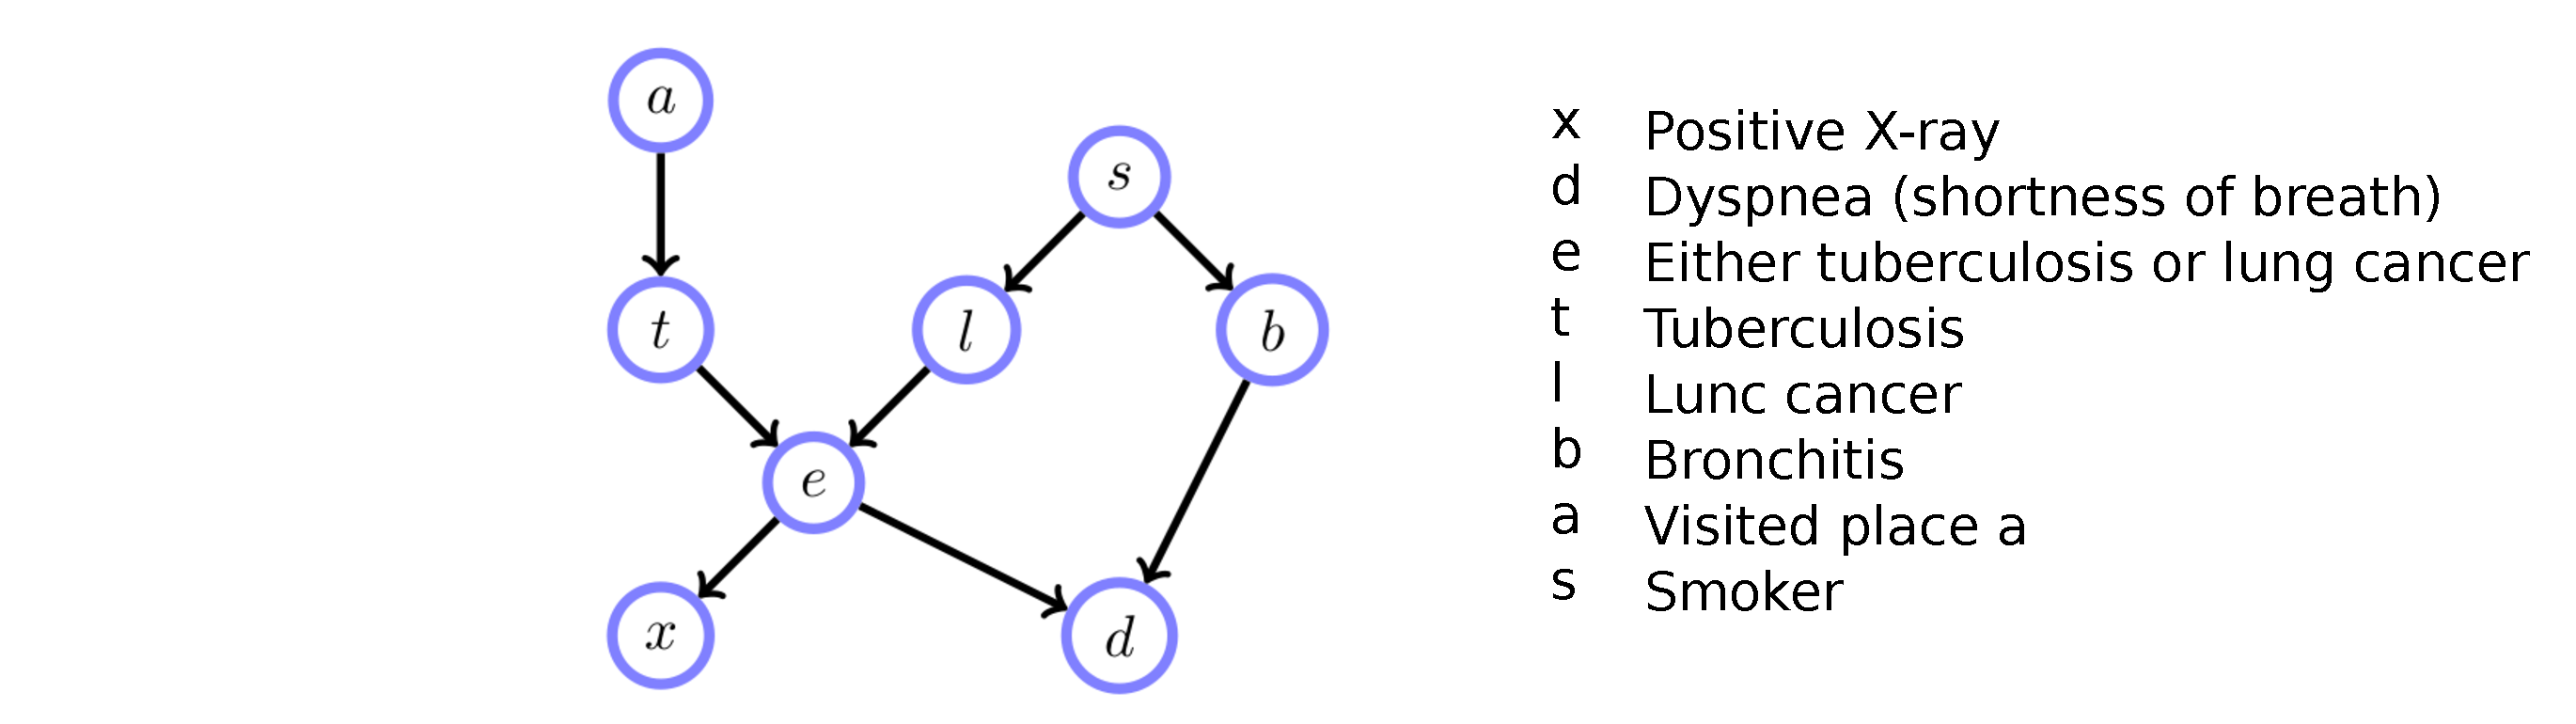
\includegraphics[width=0.9\textwidth]{chest-clinic}
  \caption{\label{fig:chest-clinic}Graphical model for \exref{ex:chest-clinic} (Barber Figure 3.15).}
\end{figure}

\begin{exenumerate}
\item Explain which of the following independence relationships hold for all distributions that factorise over the graph.
  \begin{enumerate}
  \item $t \independent s \mid d$

    \begin{solution}
      \begin{itemize}
        \item There are two trails from $t$ to $s$: $(t,e,l,s)$ and $(t,e,d,b,s)$. 
        \item The trail $(t,e,l,s)$ features a collider node $e$ that is opened by the conditioning variable $d$. The trail is thus active and we do not need to check the second trail because for independence all trails needed to be blocked.
        \item The independence relationship does thus generally not hold.
      \end{itemize}
      
      \end{solution}
    
  \item $l \independent b \mid s$

\begin{solution}
  \begin{itemize}
  \item There are two trails from $l$ to $b$: $(l,s,b)$ and $(l,e,d,b)$
  \item The trail $(l,s,b)$ is blocked by $s$ ($s$ is in a tail-tail configuration and part of the conditioning set)
  \item The trail $(l,e,d,b)$ is blocked by the collider configuration for node $d$.
  \item  All trails are blocked so that the independence relation holds.
  \end{itemize}
\end{solution}

  \end{enumerate}
  
\item Can we simplify $p(l|b,s)$ to $p(l|s)$?

  \begin{solution}
    Since $l \independent b \mid s$, we have $p(l|b,s) = p(l|s)$.
  \end{solution}

\end{exenumerate}


\ex{More on the chest clinic {\small \citep[based on][Exercise 3.3]{Barber2012}}} 
\label{ex:chest-clinic2}
Consider the directed graphical model in Figure \ref{fig:chest-clinic}.

\begin{exenumerate}
\item Explain which of the following independence relationships hold for all distributions that factorise over the graph.
  \begin{enumerate}
\item $a \independent s \mid l$
  \begin{solution}
    \begin{itemize}
      \item There are two trails from $a$ to $s$: $(a,t,e,l,s)$ and $(a,t,e,d,b,s)$
      \item The trail $(a,t,e,l,s)$ features a collider node $e$ that blocks the trail (the trail is also blocked by $l$).
      \item The trail $(a,t,e,d,b,s)$ is blocked by the collider node $d$. 
      \item All trails are blocked so that the independence relation holds.
    \end{itemize}
  \end{solution}
  
\item $a \independent s \mid l, d$

  \begin{solution}
    \begin{itemize}
      \item There are two trails from $a$ to $s$: $(a,t,e,l,s)$ and $(a,t,e,d,b,s)$
      \item The trail $(a,t,e,l,s)$ features a collider node $e$ that is opened by the conditioning variable $d$ but the $l$ node is closed by the conditioning variable $l$: the trail is blocked
      \item The trail $(a,t,e,d,b,s)$ features a collider node $d$ that is opened by conditioning on $d$. On this trail, $e$ is not in a head-head (collider) configuration) so that all nodes are open and the trail active.
      \item Hence, the independence relation does generally not hold.
    \end{itemize}
  \end{solution}          
  
  \end{enumerate}

\item Let $g$ be a (deterministic) function of $x$ and $t$. Is the expected value $\E[g(x,t) \mid l,b]$ equal to $\E[g(x,t) \mid l]$?

  \begin{solution}
    The question boils down to checking whether $x,t \independent b \mid l$. For the independence relation to hold, all trails from both $x$ and $t$ to $b$ need to be blocked by $l$.

    \begin{itemize}
      \item For $x$, we have the trails $(x,e,l,s,b)$ and $(x,e,d,b)$
      \item Trail $(x,e,l,s,b)$ is blocked by $l$
      \item Trail $(x,e,d,b)$ is blocked by the collider configuration of node $d$.
      \item For $t$, we have the trails $(t,e,l,s,b)$ and $(t,e,d,b)$
      \item Trail $(t,e,l,s,b)$ is blocked by $l$.
      \item Trail $(t,e,d,b)$ is blocked by the collider configuration of node $d$.
    \end{itemize}
    As all trails are blocked we have $x,t \independent b \mid l$ and  $\E[ g(x,t) \mid l,b] = \E[ g(x,t) \mid l]$.
    
  \end{solution}
\end{exenumerate}


\ex{Hidden Markov models}
\label{ex:HMM}
This exercise is about directed graphical models that are specified by the following DAG:
\begin{center}
  \scalebox{0.8}{
    \begin{tikzpicture}[dgraph]
      \node[cont] (y1) at (0,0) {$y_1$};
      \node[cont] (y2) at (2,0) {$y_2$};
      \node[cont] (y3) at (4,0) {$y_3$};
      \node[cont] (y4) at (6,0) {$y_4$};
      \node[cont] (x1) at (0,2) {$x_1$};
      \node[cont] (x2) at (2,2) {$x_2$};
      \node[cont] (x3) at (4,2) {$x_3$};
      \node[cont] (x4) at (6,2) {$x_4$};
      \draw(x1)--(y1);\draw(x2)--(y2);\draw(x3)--(y3);\draw(x4)--(y4);
      \draw(x1)--(x2);\draw(x2)--(x3);\draw(x3)--(x4);
  \end{tikzpicture}}
\end{center}
These models are called ``hidden'' Markov models because we typically assume to only observe the $y_i$ and not the $x_i$ that follow a Markov model.

\begin{exenumerate}
  \item Show that all probabilistic models specified by the DAG factorise as
    $$p(x_1,y_1, x_2, y_2, \ldots,x_4,y_4) = p(x_1)p(y_1|x_1)p(x_2 | x_1)p(y_2|x_2)p(x_3|x_2)p(y_3|x_3)p(x_4|x_3)p(y_4|x_4)$$
    \begin{solution}
      From the definition of directed graphical models it follows that
      $$p(x_1,y_1, x_2, y_2, \ldots,x_4,y_4) = \prod_{i=1}^4 p(x_i |
      \pa(x_i)) \prod_{i=1}^4 p(y_i | \pa(y_i)).$$ The result is then
      obtained by noting that the parent of $y_i$ is given by $x_i$ for all $i$,
      and that the parent of $x_i$ is $x_{i-1}$ for $i=2,3,4$ and that $x_1$ does not have a parent ($\pa(x_1) = \varnothing$).
    \end{solution}
%
  \item Derive the independencies implied by the ordered Markov property with the topological ordering $(x_1, y_1, x_2, y_2, x_3, y_3, x_4, y_4)$

    \begin{solution}
      $$y_i \independent x_1, y_1, \ldots, x_{i-1}, y_{i-1} \mid x_i \quad \quad  x_i \independent x_1, y_1, \ldots, x_{i-2},y_{i-2},y_{i-1} \mid x_{i-1}$$

      \end{solution}

  \item Derive the independencies implied by the ordered Markov property with the topological ordering $(x_1, x_2, \ldots, x_4, y_1, \ldots, y_4)$.
    \begin{solution} For the $x_i$, we use that for $i \ge 2$: $\pre(x_i) = \{x_1, \ldots, x_{i-1}\}$ and $\pa(x_i) = x_{i-1}$. For the $y_i$, we use that
      $\pre(y_1) = \{x_1,\ldots, x_4\}$, that $\pre(y_i) = \{x_1,\ldots, x_4, y_1, \ldots, y_{i-1}\}$ for $i>1$, and that $\pa(y_i) = x_i$. The ordered Markov property then gives:
  \begin{align*}
    x_3 \independent x_1 \mid x_2 && x_4 \independent \{x_1,x_2\} \mid x_3\\
    y_1 \independent \{x_2, x_3, x_4\} \mid x_1 &&  y_2 \independent \{x_1, x_3, x_4, y_1\} \mid x_2 \\
    y_3 \independent \{x_1, x_2, x_4, y_1, y_2\} \mid x_3 &&  y_4 \independent \{x_1, x_2, x_3, y_1, y_2, y_3\} \mid x_4
  \end{align*}

    \end{solution}

  \item Does $y_4 \independent y_1 \mid y_3$ hold?

    \begin{solution}
    The trail $y_1-x_1-x_2-x_3-x_4-y_4$ is active: none of the nodes
    is in a collider configuration, so that their default state is
    open and conditioning on $y_3$ does not block any of the nodes on
    the trail.

    While $x_1-x_2-x_3-x_4$ forms a Markov chain, where e.g.\ $x_4
    \independent x_1 \mid x_3$ holds, this not so for the distribution
    of the $y$'s.

    \end{solution}
\end{exenumerate}


\ex{Alternative characterisation of independencies}
\label{ex:independencies1}
We have seen that $x \independent y | z$ is characterised by
  $p(x,y | z) =p(x | z) p(y| z)$
  or, equivalently, by
  $p(x| y, z) = p(x | z)$.
  Show that further equivalent characterisations are
\begin{align}
  p(x,y,z) &= p(x|z) p(y|z) p(z) \quad \text{and} \label{eq:characterisation1} \\
  p(x,y,z) &= a(x,z) b(y,z) \quad \text{for some non-neg. functions \;} a(x,z) \text{\; and \;} b(x,z). \label{eq:characterisation2} 
  \end{align}
  The characterisation in Equation \eqref{eq:characterisation2} is particularly important for undirected graphical models.
\begin{solution}
  We first show the equivalence of  $p(x,y | z) =p(x | z) p(y| z)$ and
  $p(x,y,z) = p(x|z) p(y|z) p(z)$: By the product rule, we have
  $$p(x,y,z) = p(x,y|z) p(z).$$ If $p(x,y | z) =p(x | z) p(y| z)$, it
  follows that $p(x,y,z) = p(x|z) p(y|z) p(z)$. To show the opposite
  direction assume that $p(x,y,z) = p(x|z) p(y|z) p(z)$ holds. By
  comparison with the decomposition in the product rule, it follows
  that we must have $p(x,y | z) = p(x | z) p(y| z)$ whenever $p(z)>0$
  (it suffices to consider this case because for $z$ where $p(z)=0$, $p(x,y | z)$ may not be
  uniquely defined in the first place).

  Equation \eqref{eq:characterisation1} implies
  \eqref{eq:characterisation2} with $a(x,z) = p(x | z)$ and $b(y,z) =
  p(y| z)p(z)$. We now show the inverse. Let us assume that $p(x,y,z)
  = a(x,z) b(y,z)$. By the product rule, we have
  \begin{align}
    p(x,y | z)p(z) & = a(x,z) b(y,z).\\
  \end{align}
  Summing over $y$ gives
  \begin{align}
    \sum_y  p(x,y | z)p(z) & = p(z) \sum_y p(x,y | z)\\
    & = p(z) p(x|z)
  \end{align}
  Moreover
  \begin{align}
     \sum_y  p(x,y | z)p(z) & = \sum_y  a(x,z) b(y,z)\\
    & = a(x,z) \sum_y b(y,z)
  \end{align}
  so that 
  \begin{equation}
    a(x,z) = \frac{p(z) p(x | z)}{\sum_y b(y,z)}
    \label{eq:a}
  \end{equation}
  Since the sum of $p(x | z)$ over $x$ equals one we have
  \begin{equation}
    \sum_x a(x,z) = \frac{p(z)}{\sum_y b(y,z)}.
    \label{eq:asum}
  \end{equation}
  
  Now, summing $p(x,y | z) p(z)$ over $x$ yields
   \begin{align}
     \sum_x  p(x,y | z) p(z) & =  p(z) \sum_x p(x,y|z). \\
     & = p(y | z) p(z)
   \end{align}
   We also have
    \begin{align}
      \sum_x  p(x,y | z) p(z) &= \sum_x a(x,z) b(y,z) \\
      &= b(y,z) \sum_x a(x,z) \\
    &\stackrel{\eqref{eq:asum}}{=} b(y,z) \frac{p(z)}{\sum_y b(y,z)}
    \end{align}
    so that
    \begin{equation}
      p(y | z) p(z) =  p(z) \frac{b(y,z)}{\sum_y b(y,z)}
      \label{eq:brel}
    \end{equation}
   We thus have
   \begin{align}
     p(x,y,z) & = a(x,z) b(y,z) \\
     &  \stackrel{\eqref{eq:a}}{=} \frac{p(z) p(x | z)}{\sum_y b(y,z)} b(y,z) \\
     & = p(x | z)p(z) \frac{ b(y,z)}{\sum_y b(y,z)} \\
     & \stackrel{\eqref{eq:brel}}{=} p(x|z) p(y|z) p(z)
   \end{align}
   which is Equation \eqref{eq:characterisation1}.
  \end{solution}


\ex{More on independencies}
\label{ex:independencies2}
This exercise is on further properties and characterisations of statistical independence.

\begin{exenumerate}
\item Without using d-separation, show that $x \independent \{y,w\} \mid z$ implies that $x \independent y \mid z$ and $x \independent w \mid z$.\\
\emph{Hint: use the definition of statistical independence in terms of the factorisation of pmfs/pdfs.}
  
  \begin{loesung}
    We consider the joint distribution $p(x,y,w | z)$. By assumption
    \begin{equation}
      p(x,y,w | z) = p(x |z) p(y,w | z)
    \end{equation}
    We have to show that $x \independent y| z$ and $x \independent w | z$. For simplicity, we assume that the variables are discrete valued. If not, replace the sum below with an integral.

    To show that $x \independent y| z$, we marginalise $p(x,y,w | z)$
    over $w$ to obtain
    \begin{align}
      p(x,y | z ) & = \sum_w p(x,y,w | z) \\
      & = \sum_w  p(x |z) p(y,w | z) \\
      & = p(x | z) \sum_w p(y,w | z)
    \end{align}
    Since $\sum_w p(y,w | z)$ is the marginal $p(y |z)$, we have
    \begin{equation}
       p(x,y | z ) =  p(x | z) p(y | z),
    \end{equation}
    which means that $x \independent y | z$.

    To show that $x \independent w| z$, we similarly marginalise
    $p(x,y,w | z)$ over $y$ to obtain $p(x,w | z) =
    p(x|z) p(w |z)$, which means that $x \independent w | z$.
    
  \end{loesung}


\item For the directed graphical model below, show that the following two statements hold without using d-separation:

  \begin{align}
  &x \independent y \quad \text{and} \label{eq:statement1} \\
  &x \notind y \mid w \label{eq:statement2}
  \end{align}

  \begin{center}
  \scalebox{0.9}{ % x,y
    \begin{tikzpicture}[dgraph]
      \node[cont] (x) at (0,0) {$x$};
      \node[cont] (z) at (2,0) {$z$};
      \node[cont] (w) at (2,-1.5) {$w$};
      \node[cont] (y) at (4,0) {$y$};
      \draw(x) -- (z);
      \draw(y) -- (z);
      \draw(z) -- (w);
  \end{tikzpicture}}
  \end{center}
  The exercise shows that not only conditioning on a collider node but also on one of its descendents activates the trail between $x$ and $y$. You can use the result that $x \independent y |w \Leftrightarrow p(x,y,w) = a(x,w)b(y,w)$ for some non-negative functions $a(x,w)$ and $b(y,w)$.
  
  \begin{solution}
    The graphical model corresponds to the factorisation $$p(x,y,z,w) = p(x) p(y) p(z|x,y) p(w|z).$$
    For the marginal $p(x,y)$ we have to sum (integrate) over all $(z,w)$
    \begin{align}
      p(x,y) &= \sum_{z,w} p(x,y,z,w) \\
      & = \sum_{z,w} p(x) p(y) p(z|x,y) p(w|z)\\
      & = p(x) p(y) \sum_{z,w} p(z| x,y) p(w|z)\\
      & = p(x) p(y) \underbrace{\sum_{z} p(z| x,y)}_{1} \underbrace{\sum_{w} p(w|z)}_{1}\\
      & = p(x) p(y)
    \end{align}
    Since $p(x,y) = p(x) p(y)$ we have $x \independent y$.

    For $x \notind y | w$, compute $p(x,y,w)$ and use the result $x \independent y |w \Leftrightarrow p(x,y,w) = a(x,w)b(y,w)$.
    \begin{align}
      p(x,y,w) & = \sum_z p(x,y,z,w)\\
      & = \sum_z p(x) p(y) p(z|x,y) p(w|z) \\
      & = p(x) \underbrace{p(y) \sum_z p(z|x,y) p(w|z)}_{k(x,y,w)}
    \end{align}
    Since $p(x,y,w)$ cannot be factorised as $a(x,w) b(y,w)$, the relation $x \independent y | w$ cannot generally hold.
  \end{solution}

\end{exenumerate}


\ex{Independencies in directed graphical models}

Consider the following directed acyclic graph.
       \begin{center}
         \scalebox{0.9}{ % x,y
           \begin{tikzpicture}[dgraph]
             \node[cont] (x1) at (0,0) {$x_1$};
             \node[cont] (x2) at (0,-2) {$x_2$};
             \node[cont] (x3) at (0,-4) {$x_3$};
             \node[cont] (x4) at (2,-1.5) {$x_4$};
             \node[cont] (x5) at (2,-3) {$x_5$};
             \node[cont] (x6) at (2,-4.5) {$x_6$};
             \node[cont] (x7) at (4,0) {$x_7$};
             \node[cont] (x8) at (4,-2) {$x_8$};
             \node[cont] (x9) at (6,-1) {$x_9$};

             \draw (x1) -- (x2);
             \draw (x2) -- (x3);
             \draw (x1) -- (x4);
             \draw (x4) -- (x5);
             \draw (x5) -- (x6);
             \draw (x7) -- (x4);
             \draw (x7) -- (x8);
             \draw (x3) -- (x6);
             \draw (x8) -- (x6);
             \draw (x7) -- (x9);
         \end{tikzpicture}}
       \end{center}
   For each of the statements below, determine whether it holds for
   all probabilistic models that factorise over the graph. Provide a
   justification for your answer.
   
   \begin{exenumerate}
   \item  $p(x_7 | x_2) = p(x_7)$

     \begin{solution}
 Yes, it holds. $x_2$ is a non-descendant of $x_7$,
 $\pa(x_7)=\varnothing$, and hence, by the local Markov property, $x_7
 \independent x_2$, so that $p(x_7 | x_2) = p(x_7)$.
     \end{solution}
     
   \item  $x_1 \notind x_3$  

     \begin{solution}
 No, does not hold. $x_1$ and $x_3$ are d-connected, which only implies independence for \emph{some} and not all distributions that factorise over the graph. The graph generally only allows us to read out independencies and not dependencies.

     \end{solution}


   \item  $p(x_1,x_2,x_4) \propto \phi_1(x_1,x_2) \phi_2(x_1,x_4)$ for some non-negative functions $\phi_1$ and $\phi_2$. 

     \begin{solution}
       Yes, it holds. The statement is equivalent to $x_2 \independent x_4 \mid  x_1$. There are three trails from $x_2$ to $x_4$, which are all blocked:
       \begin{enumerate}
       \item $x_2-x_1-x_4$: this trail is blocked because $x_1$ is in a tail-tail connection and it is observed, which closes the node.
       \item $x_2-x_3-x_6-x_5-x_4$: this trail is blocked because
         $x_3, x_6, x_5$ is in a collider configuration, and $x_6$ is
         not observed (and it does not have any descendants).
       \item $x_2-x_3-x_6- x_8- x_7- x_4$: this trail is blocked because
         $x_3, x_6, x_8$ is in a collider configuration, and $x_6$ is
         not observed (and it does not have any descendants).
       \end{enumerate}
       Hence, by the global Markov property (d-separation), the independency holds.
     \end{solution}


   \item  $x_2 \independent x_9 \mid \{x_6, x_8\}$ 

     \begin{solution}
       No, does not hold. Conditioning on $x_6$ opens the collider node $x_4$ on the trail $x_2 - x_1 - x_4 - x_7 - x_9$, so that the trail is active.
     \end{solution}


   \item  $x_8 \independent \{x_2,x_9\} \mid \{x_3,x_5, x_6, x_7\}$ 

     \begin{solution}
       Yes, it holds. $\{x_3,x_5,x_6,x_7\}$ is the Markov blanket of $x_8$, so that $x_8$ is independent of remaining nodes given the Markov blanket.
     \end{solution}


   \item  $\E[ x_2 \cdot x_3 \cdot x_4 \cdot x_5 \cdot x_8 \mid x_7] = 0$ if $\E[x_8 \mid x_7] = 0$

     \begin{solution}
       Yes, it holds. $\{x_2,x_3,x_4,x_5\}$ are non-descendants of $x_8$, and $x_7$ is the parent of $x_8$, so that $x_8 \independent \{x_2,x_3,x_4,x_5\} \mid x_7$. This means that $\E[ x_2 \cdot x_3 \cdot x_4 \cdot x_5 \cdot x_8 \mid x_7] = \E[ x_2 \cdot x_3 \cdot x_4 \cdot x_5 \mid x_7] \E[x_8 \mid x_7] =0$.
     \end{solution}

     
   \end{exenumerate}


\ex{Independencies in directed graphical models}
  Consider the following directed acyclic graph:
   \begin{center}
     % x,y (x>0: right, y>0 up)
    \begin{tikzpicture}[dgraph]

      \node[cont] (m1) at (0,0) {$m_1$};
      \node[cont] (s1) at (2,0) {$s_1$};
      \node[cont] (u1) at (0,-1.5) {$u_1$};
      \node[cont] (v1) at (2,-1.5) {$v_1$};
      \node[cont] (x1) at (0,-3) {$x_1$};
      \node[cont] (y1) at (2,-3) {$y_1$};
      \node[cont] (theta1) at (1,-4) {$\theta_1$};
      
      \draw (m1) -- (u1);
      \draw (m1) -- (v1);
      \draw (s1) -- (u1);
      \draw (s1) -- (v1);
      \draw (u1) -- (x1);
      \draw (v1) -- (y1);
      \draw (theta1) -- (x1);
      \draw (theta1) -- (y1);

      
      \node[cont] (m2) at (4,0) {$m_2$};
      \node[cont] (s2) at (6,0) {$s_2$};
      \node[cont] (u2) at (4,-1.5) {$u_2$};
      \node[cont] (v2) at (6,-1.5) {$v_2$};
      \node[cont] (x2) at (4,-3) {$x_2$};
      \node[cont] (y2) at (6,-3) {$y_2$};
      \node[cont] (theta2) at (5,-4) {$\theta_2$};
      
      \draw (m2) -- (u2);
      \draw (m2) -- (v2);
      \draw (s2) -- (u2);
      \draw (s2) -- (v2);
      \draw (u2) -- (x2);
      \draw (v2) -- (y2);
      \draw (theta2) -- (x2);
      \draw (theta2) -- (y2);
      
      \draw (theta1) -- (theta2);
      
    \end{tikzpicture}
   \end{center}
   
    For each of the statements below, determine whether it holds for
   all probabilistic models that factorise over the graph. Provide a
   justification for your answer.
   
   \begin{exenumerate}
   \item $x_1 \independent x_2$

     \begin{solution}
       Does not hold. The trail $x_1 - \theta_1 - \theta_2 - x_2$ is
       active (unblocked) because none of the nodes is in a collider
       configuration or in the conditioning set.
     \end{solution}
     
   \item $p(x_1, y_1, \theta_1, u_1) \propto \phi_A(x_1, \theta_1, u_1)\phi_B(y_1, \theta_1, u_1)$ for some non-negative functions $\phi_A$ and $\phi_B$ 

     \begin{solution}
       Holds. The statement is equivalent to $x_1 \independent y_1
       \mid \{\theta_1, u_1\}$. The conditioning set $\{\theta_1,
       u_1\}$ blocks all trails from $x_1$ to $y_1$ because they are
       both only in serial configurations in all trails from $x_1$ to
       $y_1$, hence the independency holds by the global Markov
       property.  Alternative justification: the conditioning set is
       the Markov blanket of $x_1$, and $x_1$ and $y_1$ are not
       neighbours which implies the independency.
     \end{solution}
     
   \item $v_2 \independent \{u_1, v_1, u_2, x_2\} \mid \{m_2, s_2, y_2, \theta_2\}$

     \begin{solution}
        Holds. The conditioning set is the Markov blanket of $v_2$
        (the set of parents, children, and co-parents): the set of
        parents is $\pa(v_2)=\{m_2, s_2\}$, $y_2$ is the only child of
        $v_2$, and $\theta_2$ is the only other parent of
        $y_2$. And $v_2$ is independent of all other variables
        given its Markov blanket.
     \end{solution}

   \item $\E [ m_2 \mid  m_1 ] = \E[m_2]$

     \begin{solution}
       Holds. There are four trails from $m_1$ to $m_2$, namely via
       $x_1$, via $y_1$, via $x_2$, via $y_2$. In all trails the four
       variables are in a collider configuration, so that each of the
       trails is blocked. By the global Markov property
       (d-separation), this means that $m_1 \independent m_2$ which
       implies that $\E[m_2 \mid m_1] = \E[m_2]$.

       Alternative justification 1: $m_2$ is a non-descendent of $m_1$
       and $\pa(m_2) = \varnothing$. By the directed local Markov
       property, a variable is independent from its non-descendents
       given the parents, hence $m_2 \independent m_1$.

       Alternative justification 2: We can choose a topological
       ordering where $m_1$ and $m_2$ are the first two
       variables. Moreover, their parent sets are both empty. By the
       directed ordered Markov, we thus have $m_1 \independent m_2$.
       
     \end{solution}

     
   \end{exenumerate}

